% generated by Plantuml 1.2024.3       
\definecolor{plantucolor0000}{RGB}{255,255,255}
\definecolor{plantucolor0001}{RGB}{24,24,24}
\definecolor{plantucolor0002}{RGB}{0,0,0}
\definecolor{plantucolor0003}{RGB}{226,226,240}
\definecolor{plantucolor0004}{RGB}{238,238,238}

\begin{adjustbox}{width=.84\paperwidth, center}
	\resizebox{\textwidth}{!}{
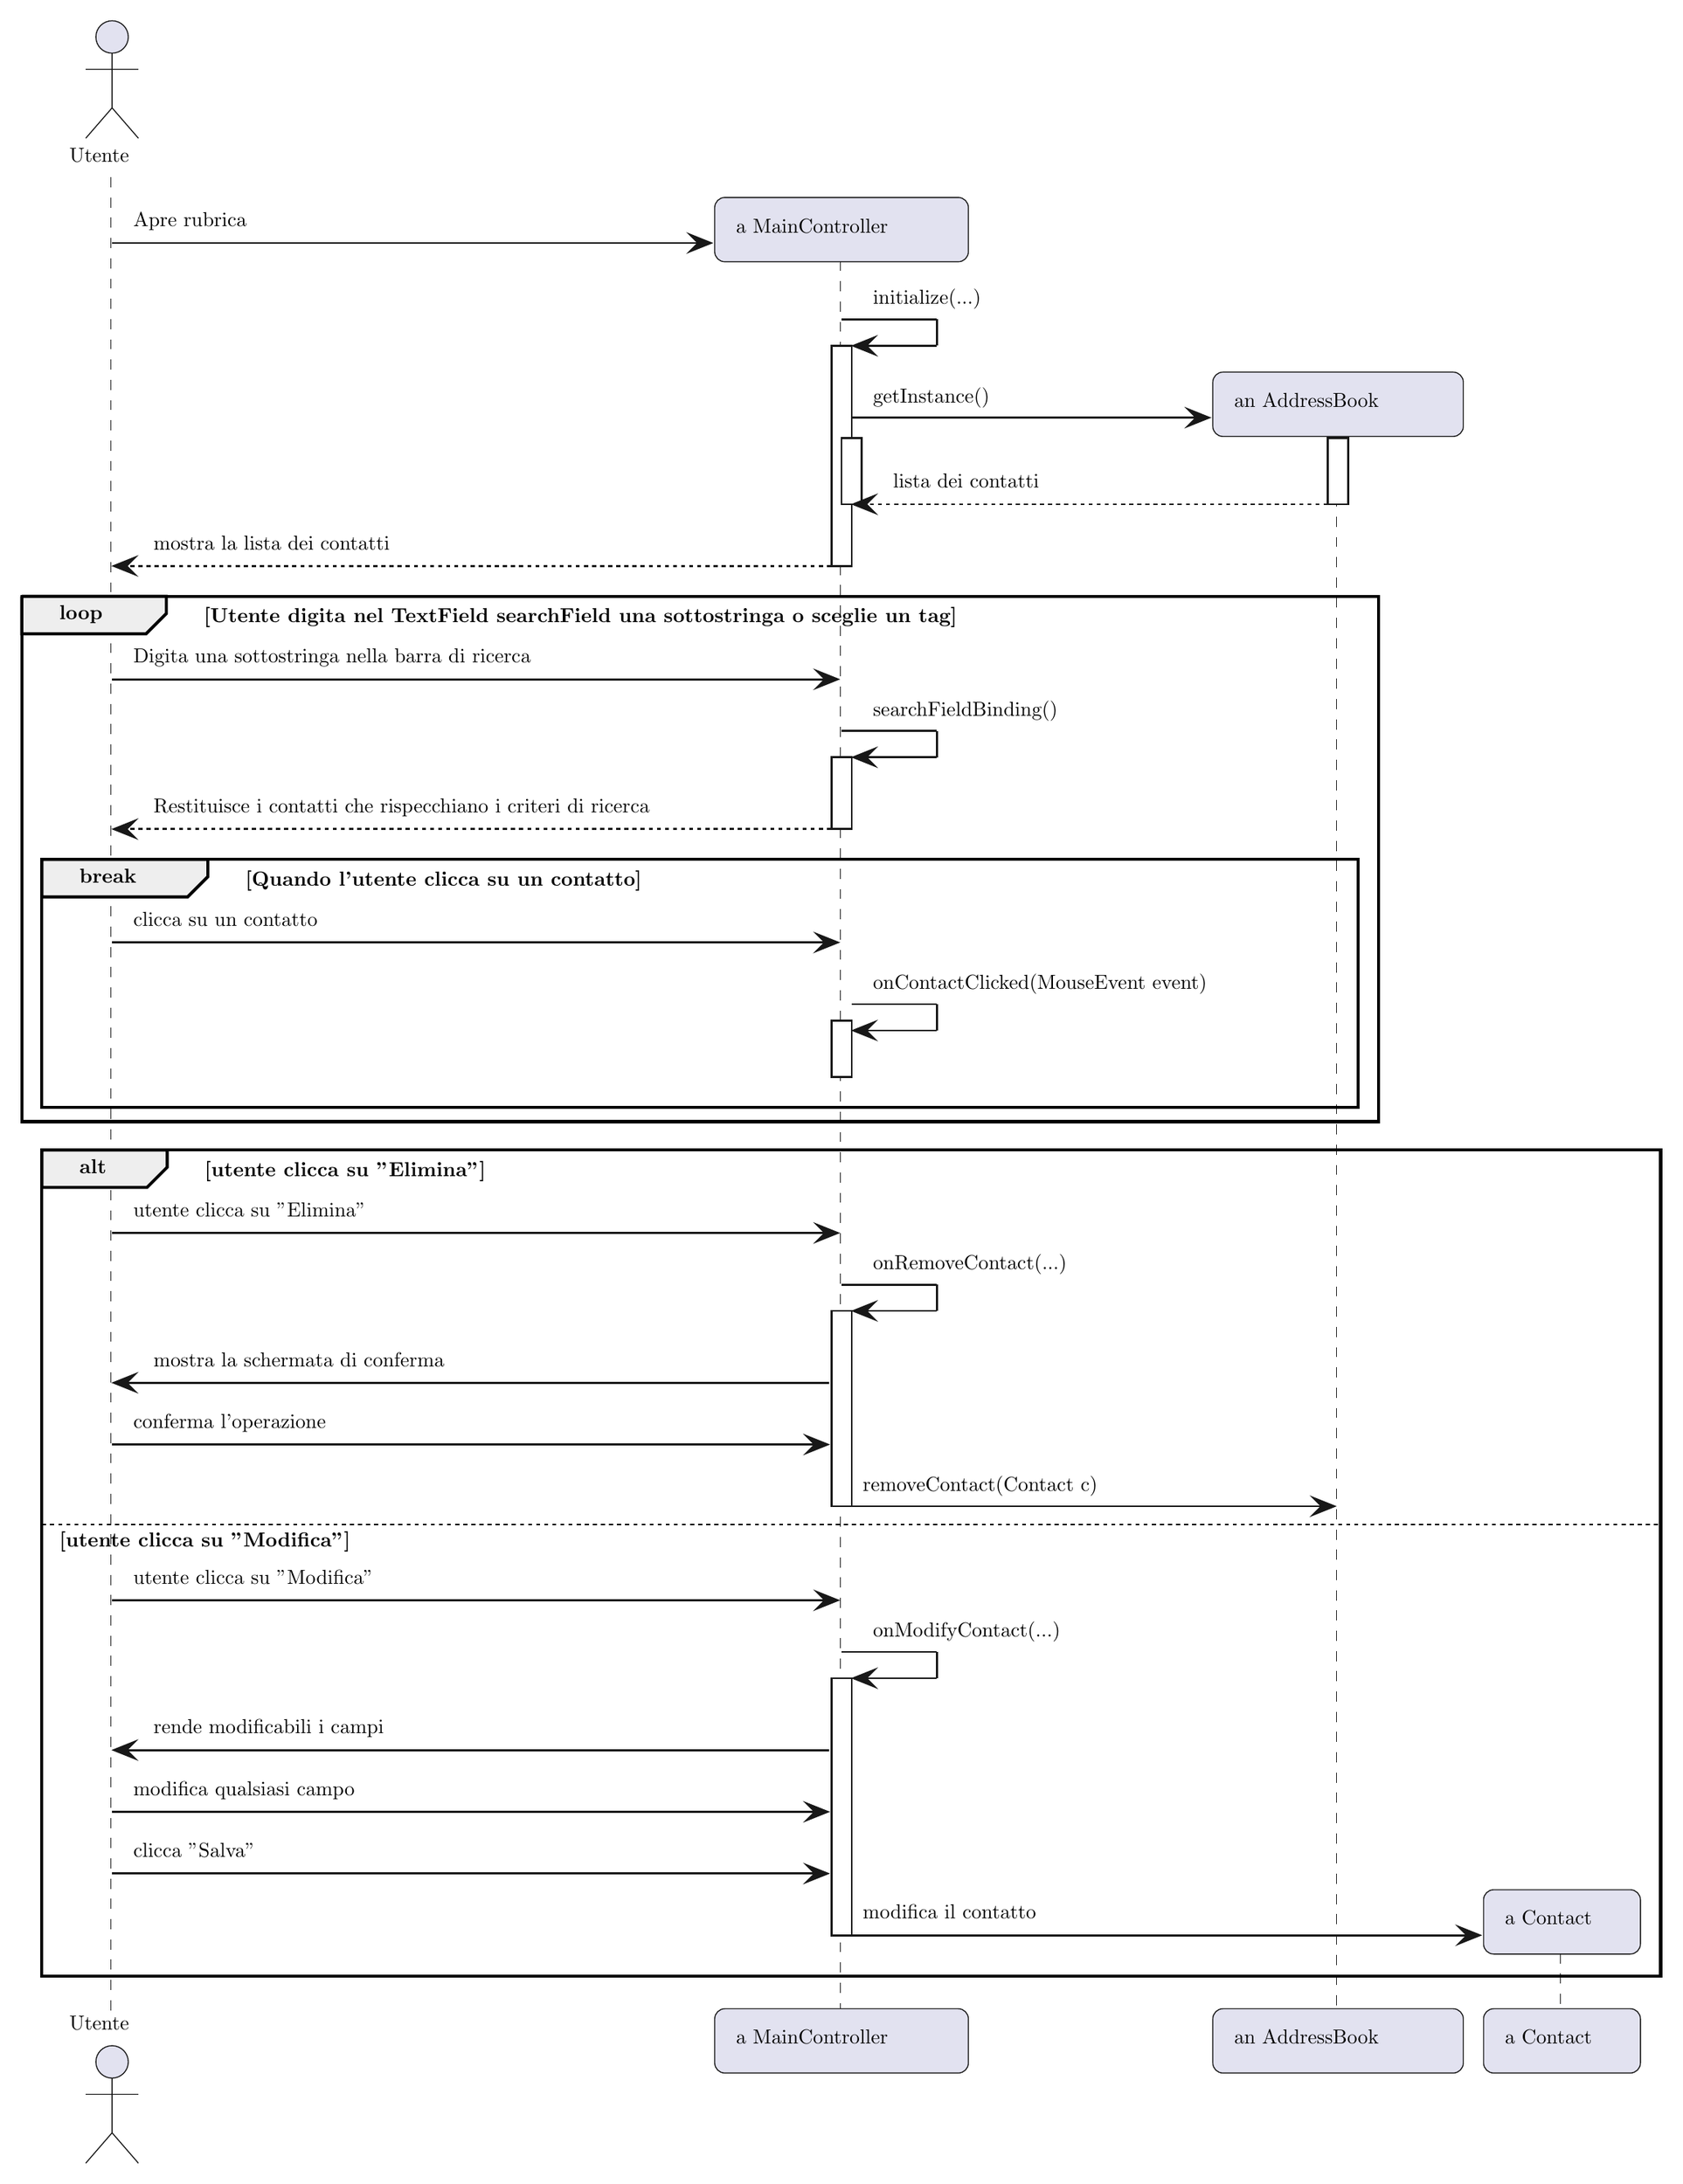
\begin{tikzpicture}[yscale=-1
,pstyle0/.style={color=plantucolor0001,fill=white,line width=1.0pt}
,pstyle1/.style={color=black,line width=1.5pt}
,pstyle2/.style={color=plantucolor0001,line width=0.5pt,dash pattern=on 5.0pt off 5.0pt}
,pstyle3/.style={color=plantucolor0001,fill=plantucolor0003,line width=0.5pt}
,pstyle4/.style={color=plantucolor0001,line width=0.5pt}
,pstyle5/.style={color=plantucolor0001,fill=plantucolor0001,line width=1.0pt}
,pstyle6/.style={color=plantucolor0001,line width=1.0pt}
,pstyle7/.style={color=plantucolor0001,line width=1.0pt,dash pattern=on 2.0pt off 2.0pt}
,pstyle8/.style={color=black,fill=plantucolor0004,line width=1.5pt}
]
\draw[pstyle0] (409.8219pt,165.9707pt) rectangle (419.8219pt,274.6738pt);
\draw[pstyle0] (414.8219pt,211.4492pt) rectangle (424.8219pt,244.1953pt);
\draw[pstyle0] (409.8219pt,369.1094pt) rectangle (419.8219pt,404.5879pt);
\draw[pstyle0] (409.8219pt,499.0234pt) rectangle (419.8219pt,527.0234pt);
\draw[pstyle0] (409.8219pt,642.459pt) rectangle (419.8219pt,738.8945pt);
\draw[pstyle0] (409.8219pt,823.7949pt) rectangle (419.8219pt,950.709pt);
\draw[pstyle0] (655.0081pt,211.4492pt) rectangle (665.0081pt,244.1953pt);
\draw[pstyle1] (10pt,289.6738pt) rectangle (680.0081pt,549.0234pt);
\draw[pstyle1] (20pt,419.5879pt) rectangle (670.0081pt,542.0234pt);
\draw[pstyle1] (20pt,563.0234pt) rectangle (819.327pt,970.9766pt);
\draw[pstyle2] (54pt,82.7461pt) -- (54pt,987.9766pt);
\draw[pstyle2] (414.1879pt,124.1191pt) -- (414.1879pt,987.9766pt);
\draw[pstyle2] (659.156pt,210.3438pt) -- (659.156pt,987.9766pt);
\draw[pstyle2] (769.8603pt,959.6035pt) -- (769.8603pt,987.9766pt);
\node at (30pt,65pt)[below right,color=black]{Utente};
\draw[pstyle3] (54.6pt,13.5pt) ellipse (8pt and 8pt);
\draw[pstyle4] (54.6pt,21.5pt) -- (54.6pt,48.5pt)(41.6pt,29.5pt) -- (67.6pt,29.5pt)(54.6pt,48.5pt) -- (41.6pt,63.5pt)(54.6pt,48.5pt) -- (67.6pt,63.5pt);
\node at (30pt,986.9766pt)[below right,color=black]{Utente};
\draw[pstyle3] (54.6pt,1013.2227pt) ellipse (8pt and 8pt);
\draw[pstyle4] (54.6pt,1021.2227pt) -- (54.6pt,1048.2227pt)(41.6pt,1029.2227pt) -- (67.6pt,1029.2227pt)(54.6pt,1048.2227pt) -- (41.6pt,1063.2227pt)(54.6pt,1048.2227pt) -- (67.6pt,1063.2227pt);
\draw[pstyle3] (352.1879pt,991.9766pt) arc (180:270:5pt) -- (357.1879pt,986.9766pt) -- (472.456pt,986.9766pt) arc (270:360:5pt) -- (477.456pt,991.9766pt) -- (477.456pt,1013.7227pt) arc (0:90:5pt) -- (472.456pt,1018.7227pt) -- (357.1879pt,1018.7227pt) arc (90:180:5pt) -- (352.1879pt,1013.7227pt) -- cycle;
\node at (359.1879pt,993.9766pt)[below right,color=black]{a MainController};
\draw[pstyle3] (598.156pt,991.9766pt) arc (180:270:5pt) -- (603.156pt,986.9766pt) -- (716.8603pt,986.9766pt) arc (270:360:5pt) -- (721.8603pt,991.9766pt) -- (721.8603pt,1013.7227pt) arc (0:90:5pt) -- (716.8603pt,1018.7227pt) -- (603.156pt,1018.7227pt) arc (90:180:5pt) -- (598.156pt,1013.7227pt) -- cycle;
\node at (605.156pt,993.9766pt)[below right,color=black]{an AddressBook};
\draw[pstyle3] (731.8603pt,991.9766pt) arc (180:270:5pt) -- (736.8603pt,986.9766pt) -- (804.327pt,986.9766pt) arc (270:360:5pt) -- (809.327pt,991.9766pt) -- (809.327pt,1013.7227pt) arc (0:90:5pt) -- (804.327pt,1018.7227pt) -- (736.8603pt,1018.7227pt) arc (90:180:5pt) -- (731.8603pt,1013.7227pt) -- cycle;
\node at (738.8603pt,993.9766pt)[below right,color=black]{a Contact};
\draw[pstyle0] (409.8219pt,165.9707pt) rectangle (419.8219pt,274.6738pt);
\draw[pstyle0] (414.8219pt,211.4492pt) rectangle (424.8219pt,244.1953pt);
\draw[pstyle0] (409.8219pt,369.1094pt) rectangle (419.8219pt,404.5879pt);
\draw[pstyle0] (409.8219pt,499.0234pt) rectangle (419.8219pt,527.0234pt);
\draw[pstyle0] (409.8219pt,642.459pt) rectangle (419.8219pt,738.8945pt);
\draw[pstyle0] (409.8219pt,823.7949pt) rectangle (419.8219pt,950.709pt);
\draw[pstyle0] (655.0081pt,211.4492pt) rectangle (665.0081pt,244.1953pt);
\draw[pstyle5] (340.1879pt,111.2246pt) -- (350.1879pt,115.2246pt) -- (340.1879pt,119.2246pt) -- (344.1879pt,115.2246pt) -- cycle;
\draw[pstyle6] (54.6pt,115.2246pt) -- (346.1879pt,115.2246pt);
\node at (61.6pt,96.7461pt)[below right,color=black]{Apre rubrica};
\draw[pstyle3] (352.1879pt,97.7461pt) arc (180:270:5pt) -- (357.1879pt,92.7461pt) -- (472.456pt,92.7461pt) arc (270:360:5pt) -- (477.456pt,97.7461pt) -- (477.456pt,119.4922pt) arc (0:90:5pt) -- (472.456pt,124.4922pt) -- (357.1879pt,124.4922pt) arc (90:180:5pt) -- (352.1879pt,119.4922pt) -- cycle;
\node at (359.1879pt,99.7461pt)[below right,color=black]{a MainController};
\draw[pstyle6] (414.8219pt,152.9707pt) -- (461.8219pt,152.9707pt);
\draw[pstyle6] (461.8219pt,152.9707pt) -- (461.8219pt,165.9707pt);
\draw[pstyle6] (420.8219pt,165.9707pt) -- (461.8219pt,165.9707pt);
\draw[pstyle5] (430.8219pt,161.9707pt) -- (420.8219pt,165.9707pt) -- (430.8219pt,169.9707pt) -- (426.8219pt,165.9707pt) -- cycle;
\node at (426.8219pt,134.4922pt)[below right,color=black]{initialize(...)};
\draw[pstyle5] (586.156pt,197.4492pt) -- (596.156pt,201.4492pt) -- (586.156pt,205.4492pt) -- (590.156pt,201.4492pt) -- cycle;
\draw[pstyle6] (419.8219pt,201.4492pt) -- (592.156pt,201.4492pt);
\node at (426.8219pt,182.9707pt)[below right,color=black]{getInstance()};
\draw[pstyle3] (598.156pt,183.9707pt) arc (180:270:5pt) -- (603.156pt,178.9707pt) -- (716.8603pt,178.9707pt) arc (270:360:5pt) -- (721.8603pt,183.9707pt) -- (721.8603pt,205.7168pt) arc (0:90:5pt) -- (716.8603pt,210.7168pt) -- (603.156pt,210.7168pt) arc (90:180:5pt) -- (598.156pt,205.7168pt) -- cycle;
\node at (605.156pt,185.9707pt)[below right,color=black]{an AddressBook};
\draw[pstyle5] (430.8219pt,240.1953pt) -- (420.8219pt,244.1953pt) -- (430.8219pt,248.1953pt) -- (426.8219pt,244.1953pt) -- cycle;
\draw[pstyle7] (424.8219pt,244.1953pt) -- (659.0081pt,244.1953pt);
\node at (436.8219pt,225.7168pt)[below right,color=black]{lista dei contatti};
\draw[pstyle5] (65.6pt,270.6738pt) -- (55.6pt,274.6738pt) -- (65.6pt,278.6738pt) -- (61.6pt,274.6738pt) -- cycle;
\draw[pstyle7] (59.6pt,274.6738pt) -- (413.8219pt,274.6738pt);
\node at (71.6pt,256.1953pt)[below right,color=black]{mostra la lista dei contatti};
\draw[pstyle8] (10pt,289.6738pt) -- (81.4pt,289.6738pt) -- (81.4pt,298.1523pt) -- (71.4pt,308.1523pt) -- (10pt,308.1523pt) -- (10pt,289.6738pt);
\draw[pstyle1] (10pt,289.6738pt) rectangle (680.0081pt,549.0234pt);
\node at (25pt,290.6738pt)[below right,color=black]{\textbf{loop}};
\node at (96.4pt,291.6738pt)[below right,color=black]{\textbf{[Utente digita nel TextField searchField una sottostringa o sceglie un tag]}};
\draw[pstyle5] (402.8219pt,326.6309pt) -- (412.8219pt,330.6309pt) -- (402.8219pt,334.6309pt) -- (406.8219pt,330.6309pt) -- cycle;
\draw[pstyle6] (54.6pt,330.6309pt) -- (408.8219pt,330.6309pt);
\node at (61.6pt,312.1523pt)[below right,color=black]{Digita una sottostringa nella barra di ricerca};
\draw[pstyle6] (414.8219pt,356.1094pt) -- (461.8219pt,356.1094pt);
\draw[pstyle6] (461.8219pt,356.1094pt) -- (461.8219pt,369.1094pt);
\draw[pstyle6] (420.8219pt,369.1094pt) -- (461.8219pt,369.1094pt);
\draw[pstyle5] (430.8219pt,365.1094pt) -- (420.8219pt,369.1094pt) -- (430.8219pt,373.1094pt) -- (426.8219pt,369.1094pt) -- cycle;
\node at (426.8219pt,337.6309pt)[below right,color=black]{searchFieldBinding()};
\draw[pstyle5] (65.6pt,400.5879pt) -- (55.6pt,404.5879pt) -- (65.6pt,408.5879pt) -- (61.6pt,404.5879pt) -- cycle;
\draw[pstyle7] (59.6pt,404.5879pt) -- (413.8219pt,404.5879pt);
\node at (71.6pt,386.1094pt)[below right,color=black]{Restituisce i contatti che rispecchiano i criteri di ricerca};
\draw[pstyle8] (20pt,419.5879pt) -- (101.9pt,419.5879pt) -- (101.9pt,428.0664pt) -- (91.9pt,438.0664pt) -- (20pt,438.0664pt) -- (20pt,419.5879pt);
\draw[pstyle1] (20pt,419.5879pt) rectangle (670.0081pt,542.0234pt);
\node at (35pt,420.5879pt)[below right,color=black]{\textbf{break}};
\node at (116.9pt,421.5879pt)[below right,color=black]{\textbf{[Quando l'utente clicca su un contatto]}};
\draw[pstyle5] (402.8219pt,456.5449pt) -- (412.8219pt,460.5449pt) -- (402.8219pt,464.5449pt) -- (406.8219pt,460.5449pt) -- cycle;
\draw[pstyle6] (54.6pt,460.5449pt) -- (408.8219pt,460.5449pt);
\node at (61.6pt,442.0664pt)[below right,color=black]{clicca su un contatto};
\draw[pstyle6] (419.8219pt,491.0234pt) -- (461.8219pt,491.0234pt);
\draw[pstyle6] (461.8219pt,491.0234pt) -- (461.8219pt,504.0234pt);
\draw[pstyle6] (420.8219pt,504.0234pt) -- (461.8219pt,504.0234pt);
\draw[pstyle5] (430.8219pt,500.0234pt) -- (420.8219pt,504.0234pt) -- (430.8219pt,508.0234pt) -- (426.8219pt,504.0234pt) -- cycle;
\node at (426.8219pt,472.5449pt)[below right,color=black]{onContactClicked(MouseEvent event)};
\draw[pstyle8] (20pt,563.0234pt) -- (81.8pt,563.0234pt) -- (81.8pt,571.502pt) -- (71.8pt,581.502pt) -- (20pt,581.502pt) -- (20pt,563.0234pt);
\draw[pstyle1] (20pt,563.0234pt) rectangle (819.327pt,970.9766pt);
\node at (35pt,564.0234pt)[below right,color=black]{\textbf{alt}};
\node at (96.8pt,565.0234pt)[below right,color=black]{\textbf{[utente clicca su "Elimina"]}};
\draw[pstyle5] (402.8219pt,599.9805pt) -- (412.8219pt,603.9805pt) -- (402.8219pt,607.9805pt) -- (406.8219pt,603.9805pt) -- cycle;
\draw[pstyle6] (54.6pt,603.9805pt) -- (408.8219pt,603.9805pt);
\node at (61.6pt,585.502pt)[below right,color=black]{utente clicca su "Elimina"};
\draw[pstyle6] (414.8219pt,629.459pt) -- (461.8219pt,629.459pt);
\draw[pstyle6] (461.8219pt,629.459pt) -- (461.8219pt,642.459pt);
\draw[pstyle6] (420.8219pt,642.459pt) -- (461.8219pt,642.459pt);
\draw[pstyle5] (430.8219pt,638.459pt) -- (420.8219pt,642.459pt) -- (430.8219pt,646.459pt) -- (426.8219pt,642.459pt) -- cycle;
\node at (426.8219pt,610.9805pt)[below right,color=black]{onRemoveContact(...)};
\draw[pstyle5] (65.6pt,673.9375pt) -- (55.6pt,677.9375pt) -- (65.6pt,681.9375pt) -- (61.6pt,677.9375pt) -- cycle;
\draw[pstyle6] (59.6pt,677.9375pt) -- (408.8219pt,677.9375pt);
\node at (71.6pt,659.459pt)[below right,color=black]{mostra la schermata di conferma};
\draw[pstyle5] (397.8219pt,704.416pt) -- (407.8219pt,708.416pt) -- (397.8219pt,712.416pt) -- (401.8219pt,708.416pt) -- cycle;
\draw[pstyle6] (54.6pt,708.416pt) -- (403.8219pt,708.416pt);
\node at (61.6pt,689.9375pt)[below right,color=black]{conferma l'operazione};
\draw[pstyle5] (648.0081pt,734.8945pt) -- (658.0081pt,738.8945pt) -- (648.0081pt,742.8945pt) -- (652.0081pt,738.8945pt) -- cycle;
\draw[pstyle6] (414.8219pt,738.8945pt) -- (654.0081pt,738.8945pt);
\node at (421.8219pt,720.416pt)[below right,color=black]{removeContact(Contact c)};
\draw[color=black,line width=1.0pt,dash pattern=on 2.0pt off 2.0pt] (20pt,747.8945pt) -- (819.327pt,747.8945pt);
\node at (25pt,747.8945pt)[below right,color=black]{\textbf{[utente clicca su "Modifica"]}};
\draw[pstyle5] (402.8219pt,781.3164pt) -- (412.8219pt,785.3164pt) -- (402.8219pt,789.3164pt) -- (406.8219pt,785.3164pt) -- cycle;
\draw[pstyle6] (54.6pt,785.3164pt) -- (408.8219pt,785.3164pt);
\node at (61.6pt,766.8379pt)[below right,color=black]{utente clicca su "Modifica"};
\draw[pstyle6] (414.8219pt,810.7949pt) -- (461.8219pt,810.7949pt);
\draw[pstyle6] (461.8219pt,810.7949pt) -- (461.8219pt,823.7949pt);
\draw[pstyle6] (420.8219pt,823.7949pt) -- (461.8219pt,823.7949pt);
\draw[pstyle5] (430.8219pt,819.7949pt) -- (420.8219pt,823.7949pt) -- (430.8219pt,827.7949pt) -- (426.8219pt,823.7949pt) -- cycle;
\node at (426.8219pt,792.3164pt)[below right,color=black]{onModifyContact(...)};
\draw[pstyle5] (65.6pt,855.2734pt) -- (55.6pt,859.2734pt) -- (65.6pt,863.2734pt) -- (61.6pt,859.2734pt) -- cycle;
\draw[pstyle6] (59.6pt,859.2734pt) -- (408.8219pt,859.2734pt);
\node at (71.6pt,840.7949pt)[below right,color=black]{rende modificabili i campi};
\draw[pstyle5] (397.8219pt,885.752pt) -- (407.8219pt,889.752pt) -- (397.8219pt,893.752pt) -- (401.8219pt,889.752pt) -- cycle;
\draw[pstyle6] (54.6pt,889.752pt) -- (403.8219pt,889.752pt);
\node at (61.6pt,871.2734pt)[below right,color=black]{modifica qualsiasi campo};
\draw[pstyle5] (397.8219pt,916.2305pt) -- (407.8219pt,920.2305pt) -- (397.8219pt,924.2305pt) -- (401.8219pt,920.2305pt) -- cycle;
\draw[pstyle6] (54.6pt,920.2305pt) -- (403.8219pt,920.2305pt);
\node at (61.6pt,901.752pt)[below right,color=black]{clicca "Salva"};
\draw[pstyle5] (719.8603pt,946.709pt) -- (729.8603pt,950.709pt) -- (719.8603pt,954.709pt) -- (723.8603pt,950.709pt) -- cycle;
\draw[pstyle6] (414.8219pt,950.709pt) -- (725.8603pt,950.709pt);
\node at (421.8219pt,932.2305pt)[below right,color=black]{modifica il contatto};
\draw[pstyle3] (731.8603pt,933.2305pt) arc (180:270:5pt) -- (736.8603pt,928.2305pt) -- (804.327pt,928.2305pt) arc (270:360:5pt) -- (809.327pt,933.2305pt) -- (809.327pt,954.9766pt) arc (0:90:5pt) -- (804.327pt,959.9766pt) -- (736.8603pt,959.9766pt) arc (90:180:5pt) -- (731.8603pt,954.9766pt) -- cycle;
\node at (738.8603pt,935.2305pt)[below right,color=black]{a Contact};
\end{tikzpicture}
}
\end{adjustbox}